\section{Analysis}\label{sec:analysis}

In this section we examine the macro-topological structure of the
unfiltered and filtered token graphs including degree distributions,
connected component structure, and cyclic structure.  We also examine
the micro-topological structure of some individual tokens.  We
visualise the composition of tokens and identify their direct and
transitive dependencies.

\begin{table}
  \centering
  \caption{Each edge in a token graph represents a set of tokenising
    meta-events.  The top five most significant edges in terms of the
    number of tokenising meta-events they contain are shown.  The
    results are the same for both the unfiltered and filtered token
    graphs, i.e., the same five edges are present in
    both.}\label{tab:most-significant-edges}
  \begin{tabular}{|c|c|r|}
    \hline

    Source Token & Target Token & \begin{tabular}{@{}c@{}}\#
      Tokenising\\Meta-Events\end{tabular}\\

    \hline

    \texttt{SHIB}~(\texttt{0x95ad61}) &
    \texttt{xSHIB}~(\texttt{0xb4a812}) & \num{402186}\\

    \texttt{BONE}~(\texttt{0x981303}) &
    \texttt{tBONE}~(\texttt{0xf7a038}) & \num{203734}\\

    \texttt{SUSHI}~(\texttt{0x6b3595}) &
    \texttt{xSUSHI}~(\texttt{0x879824}) & \num{120221}\\

    \texttt{LEASH}~(\texttt{0x27c70c}) &
    \texttt{xLEASH}~(\texttt{0xa57d31}) & \num{75180}\\

    \texttt{USDC}~(\texttt{0xa0b869}) &
    \texttt{aUSDC}~(\texttt{0xbcca60}) & \num{69373}\\

    \hline
  \end{tabular}
\end{table}

We note that each edge in a token graph represents a set of tokenising
meta-events.  Before examining the structure of the graphs, we can
identify the most significant edges in terms of the number of
tokenising meta-events they contain.
Table~\ref{tab:most-significant-edges} shows the results for both the
unfiltered and filtered token graphs.  Three of the five edges
represent the staking of memecoins
(\texttt{SHIB}~$\rightarrow$~\texttt{xSHIB},
\texttt{BONE}~$\rightarrow$~\texttt{tBONE}, and
\texttt{LEASH}~$\rightarrow$~\texttt{xLEASH}), one represents the
staking of a governance token for a decentralised exchange
(\texttt{SUSHI}~$\rightarrow$~\texttt{xSUSHI}), and one represents the
supply of a stablecoin to a decentralised lending market
(\texttt{USDC}~$\rightarrow$~\texttt{aUSDC}).  Of course, we could
also measure the significance of a edge based on, say, the volume of
tokens transacted, the present USD value of the locked tokens, etc.

\subsection{Degree Distributions}\label{sec:analysis-degree-distribution}

\begin{figure}
  \centerline{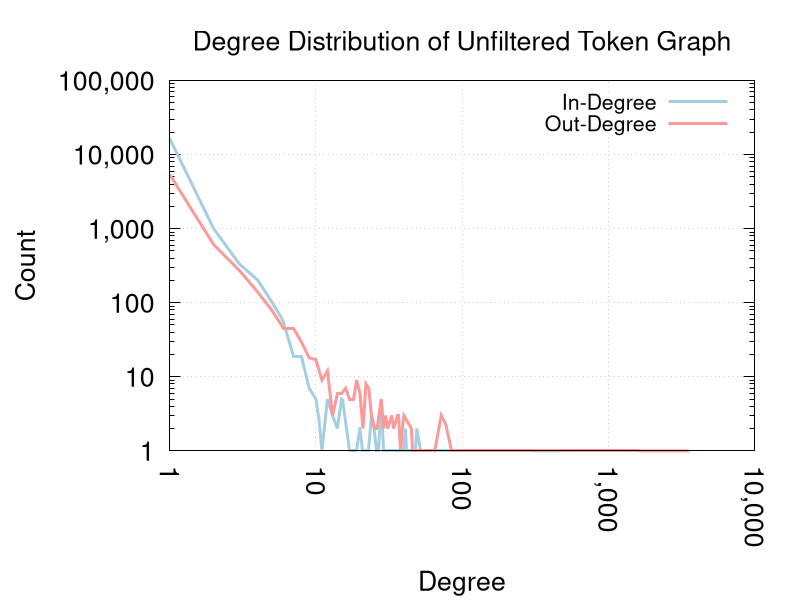
\includegraphics[width=\columnwidth]{img/degree-distributions/unfiltered-token-graph-degrees.png}}
  \caption{The in- and out-degree distributions of the unfiltered
    token graph show an inverse relationship between the degree of a
    vertex and the number of vertices with that degree in the graph.
    There are a small number of vertices with high degree and a large
    number of vertices with low
    degree.}\label{fig:unfiltered-token-graph-degrees}
\end{figure}

\begin{figure}
  \centerline{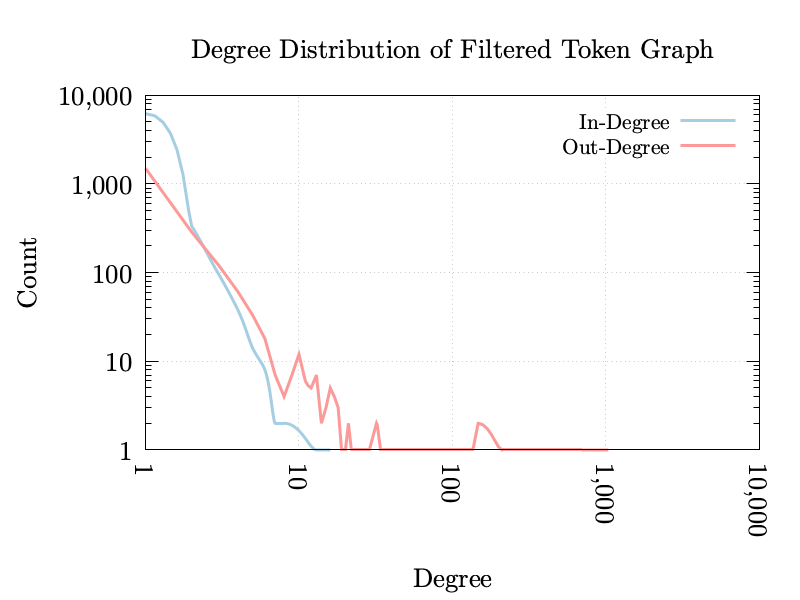
\includegraphics[width=\columnwidth]{img/degree-distributions/filtered-token-graph-degrees.png}}
  \caption{The in- and out-degree distributions of the filtered token
    graph show a similar inverse relationship as in
    Fig.~\ref{fig:unfiltered-token-graph-degrees}.}\label{fig:filtered-token-graph-degrees}
\end{figure}

\begin{table}
  \centering
  \caption{The top five vertices (tokens) in the unfiltered and
    filtered token graphs by in-degree and
    out-degree.}\label{tab:highest-in-out-degrees}
  \begin{tabular}{|c|c|r|c|r|}
    \hline

    & \multicolumn{2}{c|}{Top Five by In-Degree} &
    \multicolumn{2}{c|}{Top Five by Out-Degree}\\

    \cline{2-5}

    & Token & Deg. & Token & Deg.\\

    \hline

    \multirow{5}{0pt}{\rotatebox{90}{Unfiltered}}

    & \texttt{CHI}~(\texttt{0x000000}\footnote{The contract address
    for \texttt{CHI} is
    \texttt{0x0000000000004946c0e9f43f4dee607b0ef1fa1c}.}) & \num{471}
    & \texttt{USDC}~(\texttt{0xa0b869}) & \num{3587}\\

    & \texttt{USDP}~(\texttt{0x145668}) & \num{117} &
      \texttt{DAI}~(\texttt{0x6b1754}) & \num{1923}\\

    & \texttt{aUSDC}~(\texttt{0xbcca60}) & \num{84} &
      \texttt{USDT}~(\texttt{0xdac17f}) & \num{1175}\\

    & \texttt{aWETH}~(\texttt{0x030ba8}) & \num{63} &
      \texttt{WETH}~(\texttt{0xc02aaa}) & \num{951}\\

    & \texttt{aDAI}~(\texttt{0x028171}) & \num{54} &
      \texttt{sUSD}~(\texttt{0x57ab1e}) & \num{548}\\

    \hline

    \multirow{5}{0pt}{\rotatebox{90}{Filtered}}

    & \texttt{XDP2}~(\texttt{0xe68c1d}) & \num{16} &
    \texttt{USDC}~(\texttt{0xa0b869}) & \num{1037}\\

    & \texttt{XDP1}~(\texttt{0x134fc6}) & \num{15} &
    \texttt{DAI}~(\texttt{0x6b1754}) & \num{752}\\

    & \texttt{cyUSD}~(\texttt{0x1d0914}) & \num{14} &
    \texttt{USDT}~(\texttt{0xdac17f}) & \num{396}\\

    & \texttt{iDOL}~(\texttt{0x7591a3}) & \num{13} &
    \texttt{WETH}~(\texttt{0xc02aaa}) & \num{281}\\

    & \texttt{agEUR}~(\texttt{0x1a7e4e}) & \num{8} &
    \texttt{WBTC}~(\texttt{0x2260fa}) & \num{211}\\

    \hline
  \end{tabular}
\end{table}

The in- and out-degree distributions of the unfiltered and filtered
token graphs show an inverse relationship between the degree of a
vertex and the number of vertices with that degree in the graph (see
Fig.~\ref{fig:unfiltered-token-graph-degrees} and
Fig.~\ref{fig:filtered-token-graph-degrees}).
Table~\ref{tab:highest-in-out-degrees} shows the top five vertices in
the unfiltered and filtered token graphs by in-degree and out-degree.
The out-degree entries are easy to explain: they are the tokens that
are deposited with contracts in order to mint many other types of
tokens.  They include stablecoins (\texttt{USDC}, \texttt{DAI},
\texttt{USDT} and \texttt{sUSD}), wrapped ether (\texttt{WETH}), and
wrapped bitcoin (\texttt{WBTC}).  The in-degree entries are more
complex and have multiple explanations.  For example,
\texttt{CHI}~\cite{1inch-20} is a gas token created by 1inch, a
decentralised exchange aggregator, that is burned to obtain a
reduction in transaction fees; in some transactions the burning of
\texttt{CHI} is combined with the withdrawal of another token.  This
is a false positive generated by our heuristic since \texttt{CHI} does
not tokenise a token.  The remaining in-degree entries in the
unfiltered category are due to token swaps performed during a deposit.
For example, \texttt{aDAI}~\cite{aave-xx} is a yield-bearing token
issued by AAVE, a decentralised lending market, in exchange for the
stablecoin \texttt{DAI}.  However, in some transactions, other tokens
are supplied and swapped to \texttt{DAI}.  These are also false
positives since only \texttt{DAI} is tokenised by \texttt{aDAI}.  In
the filtered category, the in-degree entries are more reliable.  For
example, the \texttt{iDOL} token is minted when a user deposits
various forms of the \texttt{SBT} token (e.g., \texttt{SBT09180200},
\texttt{SBT09250200}, etc.) according to the Lien
Protocol~\cite{lien-20}.  Similarly, the \texttt{agEUR} token is a
stablecoin by the Angle Protocol~\cite{angle-xx} that accepts a
variety of tokens as collateral.

\begin{figure}
  \centerline{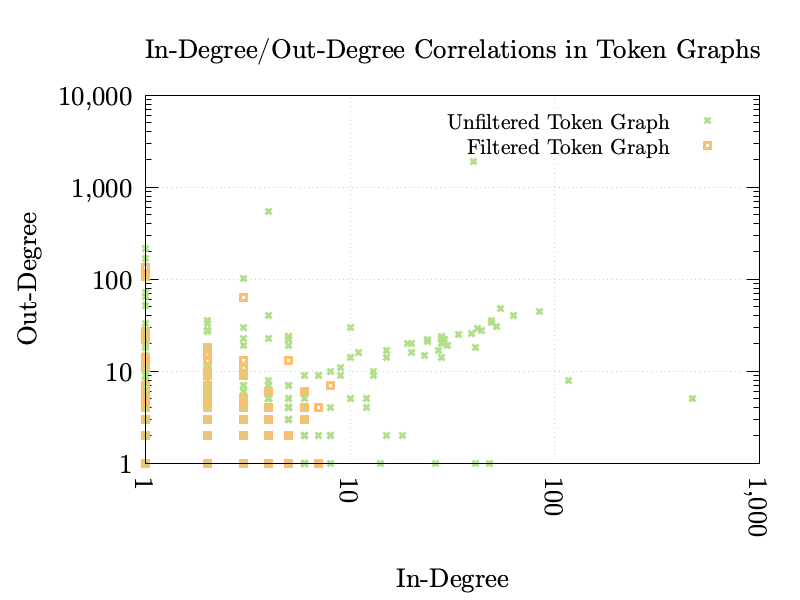
\includegraphics[width=\columnwidth]{img/degree-distributions/token-graph-in-out-degrees.png}}
  \caption{In the unfiltered and filtered token graphs, we can
    identify vertices with both high in-degree and high
    out-degree.}\label{fig:token-graph-in-out-degrees}
\end{figure}

\subsection{Connected Component Structure}\label{sec:analysis-component-structure}

\subsection{Cyclic Structure}\label{sec:analysis-cyclic-structure}

\subsection{Visualising Token Composition}\label{sec:analysis-visualisations}
